\documentclass[12pt, a4paper, portrait]{article}
\usepackage[margin = 2cm]{geometry}
\pagenumbering{gobble}
% Vertical text spacing
\parindent = 0cm \parskip = 0cm
% Section
\usepackage[compact]{titlesec} \titlespacing*{\section}{0pt}{2ex}{2ex}
\titleformat*{\section}{\normalfont\Large\bfseries\color[RGB]{0,0,192}}
% Table spacing
\newcommand\TS{\rule{0pt}{2.6ex}}         % Top strut
\newcommand\BS{\rule[-0.9ex]{0pt}{0pt}}   % Bottom strut
\usepackage{array, multirow}
\newcolumntype{L}[1]{>{\raggedright\TS\BS\arraybackslash}m{#1}}   % Align left
\newcolumntype{C}[1]{>{\centering  \TS\BS\arraybackslash}m{#1}}
\newcolumntype{R}[1]{>{\raggedleft \TS\BS\arraybackslash}m{#1}}   % Align right
% Equations
\usepackage{amsmath, bm, bbold, tikz}

\begin{document}
CO395 Group 57: Dongxiao Huang, Zheng Xun Phang, Yufeng Zhang
\section*{Implementation}
How do we select the best attribute at each node? For all attributes, we compute the information gain if the dataset is split on that attribute:
\begin{align*}
    \text{Gain(Attribute)} &= \mathcal{I}(p, n) - \left[ \frac{p_0 + n_0}{p + n} \, \mathcal{I}(p_0, n_0) + \frac{p_1 + n_1}{p + n} \, \mathcal{I}(p_1, n_1) \right] \\[0.5ex]
    p_k &= \text{Number of positive examples with attribute} = k \\
    n_k &= \text{Number of negative examples with attribute} = k \\
    p &= p_0 + p_1 = \text{Number of positive examples before split} \\
    n &= n_0 + n_1 = \text{Number of negative examples before split}
\end{align*}
There are two common ways to measure information.
\begin{flalign*}
    &\text{Entropy:} & \mathcal{I}(p, n) &= - \frac{p}{p+n} \log \frac{p}{p+n} - \frac{n}{p+n} \log \frac{n}{p+n} \qquad \text{if } p, n \neq 0 &\\
    & & \mathcal{I}(p, 0) &= \mathcal{I}(0, n) = 0 &\\[0.5ex]
    &\text{Gini impurity:} & \mathcal{I}(p, n) &= \frac{p}{p+n} \left( 1 - \frac{p}{p+n} \right) + \frac{n}{p+n} \left( 1 - \frac{n}{p+n} \right)
\end{flalign*}
We used entropy since it's stated in the specification, but Gini impurity is faster to compute. Both metrics should give similar results since their graphs have a similar shape:
\begin{center}
\begin{minipage} {0.45 \textwidth}
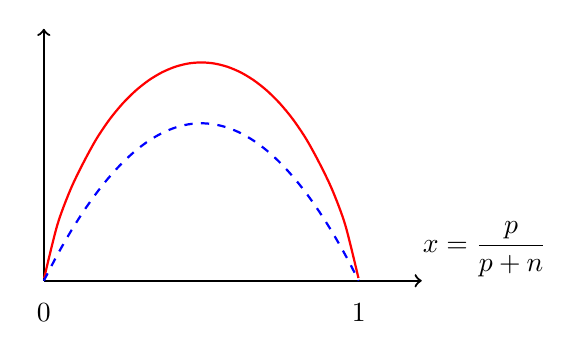
\begin{tikzpicture} [xscale = 4, yscale = 4]
    \draw[->, thick] (0, 0) -- (1.2, 0); 
    \node at (1.4, 0.1) {$\displaystyle x = \frac{p}{p+n}$};
    \draw[->, thick] (0, 0) -- (0, 0.8);
    \newcommand{\gini}[2]    {plot[smooth, domain = #1:#2] (\x, {2 * \x * (1-\x)}) };
    \newcommand{\entropy}[2] {plot[smooth, domain = #1:#2] (\x, {-\x * ln(\x) - (1-\x) * ln(1-\x)}) };
    \draw[thick, red] \entropy{0.001}{0.999};
    \draw[dashed, thick, blue] \gini{0}{1};
    \node at (0, -0.1) {0};
    \node at (1, -0.1) {1};
\end{tikzpicture}
\end{minipage}
\begin{minipage} [b] {0.4 \textwidth}
    {\color{red} Entropy: $-x \log x - (1-x) \log (1-x)$} \\
    \\
    {\color{blue} Gini: $2x (1-x)$}
\end{minipage}
\end{center}
N.B. The \textit{height} of those graphs is irrelevant because minimizing a function is equivalent to minimizing any positive multiple of that function. What matters is their \textit{shape}.\par
\bigskip
The decision tree algorithm is given in the specification, so it's unnecessary to repeat it here. We try to use NumPy functions instead of Python loops for performance since the former run on vectorized C code.\par
\bigskip
To evaluate our decision tree, we performed $K$-fold cross validation as follows:
\begin{enumerate}
    \item Shuffle the dataset and split it into $K = 10$ parts
    \item For each $k \in \{1, \dotsm, K\}$ we train the decision tree on the dataset \textit{excluding} part $k$ and then test the decision tree on part $k$. During testing, the relevant cells in the confusion matrix are incremented.
\end{enumerate}

\section*{Evaluation}
Each cell of the confusion matrix is a total, not an average, over \textit{all} folds of cross validation.
\begin{center}
\begin{tabular} { C{1.8cm} | C{1.5cm} C{1.5cm} C{1.3cm} C{1.7cm} C{1.5cm} C{1.5cm} }
    \multirow{2}{*}{Predicted} &
    \multicolumn{6}{c}{Actual} \\
    & Anger & Disgust & Fear & Happiness & Sadness & Surprise \\ \hline
    Anger     & 106 &  11 &  3 &   5 &  5 &   1 \\
    Disgust   &  23 & 157 &  1 &   5 &  9 &   3 \\
    Fear      &  17 &   2 & 77 &   2 &  7 &  13 \\
    Happiness &  22 &   6 &  1 & 179 &  6 &   1 \\
    Sadness   &  34 &  11 &  3 &   4 & 78 &   2 \\
    Surprise  &  27 &   3 &  7 &   4 &  4 & 161
\end{tabular}
\end{center}
We add up the relevant cells in the confusion matrix above to compute these summary statistics:
\begin{center}
\begin{tabular} { C{2.5cm} | C{1.5cm} C{1.5cm} C{1.3cm} C{1.7cm} C{1.5cm} C{1.5cm} }
    & Anger & Disgust & Fear & Happiness & Sadness & Surprise \\ \hline
    Precision   &   &   &   &   &   &   \\
    Recall      &   &   &   &   &   &   \\
    $F_1$ score &   &   &   &   &   &   \\
    Classification rate &   &   &   &   &   &
\end{tabular}
\end{center}
Our 6 trees classify the emotions `   ', `   ' with high accuracy while `   ' seem harder to recognize.

\section*{Miscellaneous}
\textit{Noisy-Clean Datasets Question}\par
\bigskip
The noisy dataset has lower performance.\par
\bigskip
\textit{Ambiguity Question}\par
\bigskip
In case our 6 trees predict that a given image depicts more than one emotion, we considered several methods of selecting only one emotion:\par
\bigskip
1. Select at random e.g. select the first emotion in alphabetical order\par
\bigskip
2. Disable each active unit in turn, and take a majority vote\par
Example:\par
\bigskip
\textit{Pruning Question}\par
\bigskip
\end{document}
